\documentclass[crop, tikz]{standalone}
\usepackage{tikz}

\usepackage{bm}
\usepackage{relsize}
\usepackage{pgfplots}
 
\usetikzlibrary{arrows,shapes, decorations.pathmorphing,backgrounds,positioning}

\begin{document}
\begin{tikzpicture}
	\node[rectangle, rounded corners=10, minimum width=20em, minimum height=12em, draw, very thick] (lstm) at (0, 0) {};
	
	
	\node[rectangle, rounded corners=10, minimum width=5em, minimum height=3em, draw, very thick] (lst2) at (-1.5, -5.5) {};
	
	\node[rectangle, rounded corners=10, minimum width=5em, minimum height=3em, draw, very thick,left=1em of lst2] (lst1) {};
	
	\node[rectangle, rounded corners=10, minimum width=5em, minimum height=3em, draw, very thick,right=1em of lst2] (lst3) {};
	
	\node[right=0.5em of lst3] (dots) {};
	
	\node[rectangle, rounded corners=10, minimum width=5em, minimum height=3em, draw, very thick,right=3em of lst3] (lst4) {};
	
	\node[rectangle, minimum width=27em, minimum height=5.1em, ultra thick, draw] at (-0.1, -5.5) (chn1) {};
	\begin{scope}[transparency group, opacity=0.5]
	\draw[-stealth, line width=4mm] ([xshift=+1em]chn1.west) -- ([xshift=-1em]chn1.east);
	\end{scope}
	
	\node[below=2em of lst1] (x1) {$x_1$};
	\node[below=2em of lst2] (x2) {$x_2$};
	\node[below=2em of lst3] (x3) {$x_3$};
	\node[below=3.4em of dots] (xd) {\dots};
	\node[below=2em of lst4] (x4) {$x_n$};
	\node[above=2em of lst1] (y1) {$y_1$};
	\node[above=2em of lst2] (y2) {$y_2$};
	\node[above=2em of lst3] (y3) {$y_3$};
	\node[above=3.4em of dots] (yd) {\dots};
	\node[above=2em of lst4] (y4) {$y_n$};
	
	\draw[-stealth, line width=1mm, white] (x1) -- (lst1);
	\draw[-stealth, line width=1mm, white] (x2) -- (lst2);
	\draw[-stealth, line width=1mm, white] (x3) -- (lst3);
	\draw[-stealth, line width=1mm, white] (x4) -- (lst4);
	\draw[-stealth, very thick] (x1) -- (lst1);
	\draw[-stealth, very thick] (x2) -- (lst2);
	\draw[-stealth, very thick] (x3) -- (lst3);
	\draw[-stealth, very thick] (x4) -- (lst4);
	
	\draw[-stealth, line width=1mm, white] (lst1) -- (y1);
	\draw[-stealth, line width=1mm, white] (lst2) -- (y2);
	\draw[-stealth, line width=1mm, white] (lst3) -- (y3);
	\draw[-stealth, line width=1mm, white] (lst4) -- (y4);
	\draw[-stealth, very thick] (lst1) -- (y1);
	\draw[-stealth, very thick] (lst2) -- (y2);
	\draw[-stealth, very thick] (lst3) -- (y3);
	\draw[-stealth, very thick] (lst4) -- (y4);
	
	\draw[-stealth, very thick] ([yshift=-0.5em]lst1.east) -- ([yshift=-0.5em]lst2.west);
	\draw[-stealth, very thick] ([yshift=+0.5em]lst1.east) -- ([yshift=+0.5em]lst2.west);
	\draw[-stealth, very thick] ([yshift=-0.5em]lst2.east) -- ([yshift=-0.5em]lst3.west);
	\draw[-stealth, very thick] ([yshift=+0.5em]lst2.east) -- ([yshift=+0.5em]lst3.west);
	\draw[-stealth, dashed, very thick] ([yshift=-0.5em]lst3.east) -- ([yshift=-0.5em]lst4.west);
	\draw[-stealth, dashed, very thick] ([yshift=+0.5em]lst3.east) -- ([yshift=+0.5em]lst4.west);
	
	\node[rectangle, minimum width=3em, minimum height=7em, ultra thick, draw] at (-3, -9.5) (chn2) {};
	\draw[-stealth, line width=3mm, black!50] ([yshift=-1em]chn2.north) -- ([yshift=+1em]chn2.south);
	
	\node[rectangle, minimum width=3em, minimum height=7em, ultra thick, below=5.5em of chn2, draw] (chn22) {};
	\draw[-stealth, line width=3mm, black!50] ([yshift=-1em]chn22.north) -- ([yshift=+1em]chn22.south);
	
	\node[rectangle, minimum width=3em, minimum height=7em, ultra thick, right=3em of chn2, draw] (chn3) {};
	\draw[-stealth, line width=3mm, black!50] ([yshift=-1em]chn3.north) -- ([yshift=+1em]chn3.south);
	\node[rectangle, minimum width=3em, minimum height=7em, ultra thick, right=-0.2em of chn3, draw] (chn31) {};
	\draw[-stealth, line width=3mm, black!50] ([yshift=-1em]chn31.north) -- ([yshift=+1em]chn31.south);
	
	\node[rectangle, minimum width=3em, minimum height=7em, ultra thick, right=3em of chn22, draw] (chn23) {};
	\draw[-stealth, line width=3mm, black!50] ([yshift=-1em]chn23.north) -- ([yshift=+1em]chn23.south);
	\node[rectangle, minimum width=3em, minimum height=7em, ultra thick, right=-0.2em of chn23, draw] (chn231) {};
	\draw[-stealth, line width=3mm, black!50] ([yshift=-1em]chn231.north) -- ([yshift=+1em]chn231.south);
	
	
	\node[rectangle, minimum width=3em, minimum height=7em, ultra thick, right=3em of chn31, draw] (chn4) {};
	\draw[-stealth, line width=3mm, black!50] ([yshift=-1em]chn4.north) -- ([yshift=+1em]chn4.south);
	
	
	
	\node[rectangle, minimum width=3em, minimum height=7em, ultra thick, right=3em of chn231, draw] (chn24) {};
	\draw[-stealth, line width=3mm, black!50] ([yshift=-1em]chn24.north) -- ([yshift=+1em]chn24.south);
	
	\draw[-stealth, very thick] ([xshift=-3em,yshift=-2em]chn2.west) -- ([yshift=-2em]chn2.west);
	\draw[-stealth, very thick] ([xshift=-3em,yshift=2em]chn2.west) -- ([yshift=2em]chn2.west);
	\draw[-stealth, very thick] ([xshift=-3em]chn2.west) -- (chn2.west);
	
	
	\draw[-stealth, very thick] ([yshift=-2em]chn2.east) -- ([yshift=-2em]chn3.west);
	\draw[-stealth, very thick] ([yshift=2em]chn2.east) -- ([yshift=2em]chn3.west);
	\draw[-stealth, very thick] (chn2.east) -- (chn3.west);
	
	\draw[-stealth, very thick] ([yshift=-2em]chn31.east) -- ([yshift=-2em]chn4.west);
	\draw[-stealth, very thick] ([yshift=2em]chn31.east) -- ([yshift=2em]chn4.west);
	\draw[-stealth, very thick] (chn31.east) -- (chn4.west);
	
	
	\draw[-stealth, very thick] ([yshift=-2em]chn4.east) -- ([yshift=-2em,xshift=3em]chn4.east) node[right] {\dots};
	
	\draw[-stealth, very thick] ([xshift=-3em,yshift=-2em]chn22.west) -- ([yshift=-2em]chn22.west);
	\draw[-stealth, very thick] ([xshift=-3em,yshift=2em]chn22.west) -- ([yshift=2em]chn22.west);
	\draw[-stealth, very thick] ([xshift=-3em]chn22.west) -- (chn22.west);
	
	
	\draw[-stealth, very thick] ([yshift=-2em]chn22.east) -- ([yshift=-2em]chn23.west);
	\draw[-stealth, very thick] ([yshift=2em]chn22.east) -- ([yshift=2em]chn23.west);
	\draw[-stealth, very thick] (chn22.east) -- (chn23.west);
	
	\draw[-stealth, decoration={snake, pre length=0.01mm, segment length=2mm, amplitude=0.3mm, post length=1.5mm}, decorate,very thick] ([yshift=-2em]chn2.east) -- ([yshift=-2em]chn231.west);
	\draw[-stealth, decoration={snake, pre length=0.01mm, segment length=2mm, amplitude=0.3mm, post length=1.5mm}, decorate,very thick] ([yshift=2em]chn2.east) -- ([yshift=2em]chn231.west);
	\draw[-stealth, decoration={snake, pre length=0.01mm, segment length=2mm, amplitude=0.3mm, post length=1.5mm}, decorate,very thick] (chn2.east) -- (chn231.west);
	
	\draw[-stealth, decoration={snake, pre length=0.01mm, segment length=2mm, amplitude=0.3mm, post length=1.5mm}, decorate,very thick] ([yshift=-2em]chn22.east) -- ([yshift=-2em]chn31.west);
	\draw[-stealth, decoration={snake, pre length=0.01mm, segment length=2mm, amplitude=0.3mm, post length=1.5mm}, decorate,very thick] ([yshift=2em]chn22.east) -- ([yshift=2em]chn31.west);
	\draw[-stealth, decoration={snake, pre length=0.01mm, segment length=2mm, amplitude=0.3mm, post length=1.5mm}, decorate,very thick] (chn22.east) -- (chn31.west);
	
	\draw[-stealth, decoration={snake, pre length=0.01mm, segment length=2mm, amplitude=1mm, post length=1.5mm}, decorate,very thick] ([yshift=-2em]chn31.east) -- ([yshift=-2em]chn4.west);
	\draw[-stealth, decoration={snake, pre length=0.01mm, segment length=2mm, amplitude=1mm, post length=1.5mm}, decorate,very thick] ([yshift=2em]chn31.east) -- ([yshift=2em]chn4.west);
	\draw[-stealth, decoration={snake, pre length=0.01mm, segment length=2mm, amplitude=1mm, post length=1.5mm}, decorate,very thick] (chn31.east) -- (chn4.west);
	
		\draw[-stealth, decoration={snake, pre length=0.01mm, segment length=2mm, amplitude=1mm, post length=1.5mm}, decorate,very thick] ([yshift=-2em]chn231.east) -- ([yshift=-2em]chn24.west);
	\draw[-stealth, decoration={snake, pre length=0.01mm, segment length=2mm, amplitude=1mm, post length=1.5mm}, decorate,very thick] ([yshift=2em]chn231.east) -- ([yshift=2em]chn24.west);
	\draw[-stealth, decoration={snake, pre length=0.01mm, segment length=2mm, amplitude=1mm, post length=1.5mm}, decorate,very thick] (chn231.east) -- (chn24.west);
	
	\draw[-stealth, very thick] ([yshift=-2em]chn231.east) -- ([yshift=-2em]chn24.west);
	\draw[-stealth, very thick] ([yshift=2em]chn231.east) -- ([yshift=2em]chn24.west);
	\draw[-stealth, very thick] (chn231.east) -- (chn24.west);
	
	
	\draw[-stealth, very thick] ([yshift=-2em]chn24.east) -- ([yshift=-2em,xshift=3em]chn24.east) node[right] {\dots};
	
	\draw[densely dotted, very thick] (chn1.north west) -- (chn2.north east);
	\draw[densely dotted, very thick] (chn1.north east) -- (chn2.south east);
	\draw[densely dotted, very thick] (chn1.south west) -- (chn2.north west);
	\draw[densely dotted, very thick] (chn1.south east) -- (chn2.south west);
	
	\node[rectangle, minimum width=27em, minimum height=5.1em, ultra thick, draw, fill=white] at (-0.1, -5.5) (chn1) {};
	
	\draw[densely dotted, very thick] ([xshift=0.4em,yshift=-0.4em]lstm.north west) -- ([xshift=0.4em,yshift=-0.4em]lst2.north west);
	
	\draw[densely dotted, very thick] ([xshift=-0.4em,yshift=-0.4em]lstm.north east) -- ([xshift=-0.4em,yshift=-0.4em]lst2.north east);
	
	\draw[densely dotted, very thick] ([xshift=-0.4em,yshift=0.4em]lstm.south east) -- ([xshift=-0.4em,yshift=0.4em]lst2.south east);
	
	\draw[densely dotted, very thick] ([xshift=0.4em,yshift=0.4em]lstm.south west) -- ([xshift=0.4em,yshift=0.4em]lst2.south west);
	
	\node[rectangle, rounded corners=10, minimum width=20em, minimum height=12em, draw, very thick, fill=white] (lstm) at (0, 0) {};
	
	\node[rectangle, draw] at (-2.5, -0.8) (s1) {\begin{tikzpicture} \begin{axis}[
			samples=1000, domain=-2.6:2.6,
				hide axis,
				xtick=\empty,
				ytick=\empty,
				xlabel=\empty,
				ylabel=\empty,
				xmin=-2.1, xmax=2.1,
				ymin=-0.1, ymax=1.1,
				x=0.5em, y=0.5em,
				trig format = rad
			]
				\addplot expression [no markers, smooth, thick, black] {max(0, min(1, x*0.6 + 0.5))};
			\end{axis}\end{tikzpicture}};
	\node[rectangle, draw, right=1em of s1] (s2) {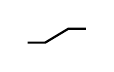
\begin{tikzpicture} \begin{axis}[
			samples=1000, domain=-2.6:2.6,
				hide axis,
				xtick=\empty,
				ytick=\empty,
				xlabel=\empty,
				ylabel=\empty,
				xmin=-2.1, xmax=2.1,
				ymin=-0.1, ymax=1.1,
				x=0.5em, y=0.5em,
				trig format = rad
			]
				\addplot expression [no markers, smooth, thick, black] {max(0, min(1, x*0.6 + 0.5))};
			\end{axis}\end{tikzpicture}};
	\node[rectangle, draw, right=1em of s2] (t1) {
\begin{tikzpicture} \begin{axis}[
			samples=1000, domain=-2.6:2.6,
				hide axis,
				xtick=\empty,
				ytick=\empty,
				xlabel=\empty,
				ylabel=\empty,
				xmin=-2.1, xmax=2.1,
				ymin=-1.1, ymax=1.1,
				x=0.5em, y=0.5em,
				trig format = rad
			]
				\addplot expression [no markers, smooth, thick, black] {tanh(\x)};
			\end{axis}\end{tikzpicture}};
	\node[rectangle, draw, right=1em of t1] (s3) {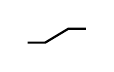
\begin{tikzpicture} \begin{axis}[
			samples=1000, domain=-2.6:2.6,
				hide axis,
				xtick=\empty,
				ytick=\empty,
				xlabel=\empty,
				ylabel=\empty,
				xmin=-2.1, xmax=2.1,
				ymin=-0.1, ymax=1.1,
				x=0.5em, y=0.5em,
				trig format = rad
			]
				\addplot expression [no markers, smooth, thick, black] {max(0, min(1, x*0.6 + 0.5))};
			\end{axis}\end{tikzpicture}};
	\node[circle, draw, above=2em of t1, inner sep=0em] (m1) {$\otimes$};
	\node[circle, draw, above=6em of s1, inner sep=0em] (m2) {$\otimes$};
	\node[circle, draw, right=6.55em of m2, inner sep=0em] (p1) {$\oplus$};
	\node[circle, draw, right=4.5em of m1, inner sep=0em] (m3) {$\otimes$};
	\node[rounded rectangle, draw, above=1em of m3, inner sep=0.2em] (tt) {
\begin{tikzpicture} \begin{axis}[
			samples=1000, domain=-2.6:2.6,
				hide axis,
				xtick=\empty,
				ytick=\empty,
				xlabel=\empty,
				ylabel=\empty,
				xmin=-2.1, xmax=2.1,
				ymin=-1.1, ymax=1.1,
				x=0.5em, y=0.5em,
				trig format = rad
			]
				\addplot expression [no markers, smooth, thick, black] {tanh(\x)};
			\end{axis}\end{tikzpicture}};
	
	\node[circle, draw, below=1em of s1, inner sep=0em] (conc) {$||$};
	
	\node[below=5em of s1] (xt) {$x_t$};
	\node[left=3em of conc] (ht1) {$y_{t-1}$};
	\node[left=3em of m2] (ct1) {$c_{t-1}$};
	\node[right=18em of m2] (ct) {$c_t$};
	\node[right=18em of conc] (ht) {$y_t$};
	\node[] (yt) at (3, 3) {$y_t$};
	
	\draw[-stealth, line width=1mm, white] (xt) -- (conc);
	\draw[-stealth, very thick] (xt) -- (conc);
	\draw[-stealth, line width=1mm, white] (ht1) -- (conc);
	\draw[-stealth, very thick] (ht1) -- (conc);
	
	\draw[-stealth, very thick] (conc) -- (s1);
	\path[-stealth, very thick] (conc) edge[bend right] (s2.south);
	\path[-stealth, very thick] (conc) edge[bend right] (t1.south);
	\path[-stealth, very thick] (conc) edge[bend right] (s3.south);
	\draw[-stealth, very thick] (s1) -- node[left] {$f_t$} (m2);
	\draw[-stealth, very thick] (s2) edge[bend left] node[above] {$j_t$} (m1.west);
	\draw[-stealth, very thick] (t1) -- node[right] {$i_t$} (m1);
	\draw[-stealth, very thick] (m1) -- (p1);
	\draw[-stealth, line width=1mm, white] (ct1) -- (m2);
	\draw[-stealth, very thick] (ct1) -- (m2);
	\draw[-stealth, very thick] (m2) -- (p1);
	\draw[-stealth, very thick] (s3) edge[bend left] node[left] {$o_t$} (m3.west);
	
	\draw[-stealth, line width=1mm, white] (p1) -- (ct);
	\draw[-stealth, very thick] (p1) -- (ct);
	\draw[-stealth, very thick] (tt) -- (m3);
	\draw[-stealth, line width=1mm, white] (m3) edge[bend right] (ht.west);
	\draw[-stealth, very thick] (m3) edge[bend right] (ht.west);
	
	\draw[-stealth ,very thick] (p1) edge[bend right] (tt.west);
	\draw[-stealth, line width=1mm,white] (m3) edge[bend right] (yt.south);
	\draw[-stealth, very thick] (m3) edge[bend right] (yt.south);
	
	\node[rectangle, rounded corners=10, minimum width=5em, minimum height=3em, draw, very thick] (lst2) at (-1.5, -5.5) {};
	
	\node[rectangle, rounded corners=10, minimum width=5em, minimum height=3em, draw, very thick,left=1em of lst2] (lst1) {};
	
	\node[rectangle, rounded corners=10, minimum width=5em, minimum height=3em, draw, very thick,right=1em of lst2] (lst3) {};
	
	\node[right=0.5em of lst3] (dots) {};
	
	\node[rectangle, rounded corners=10, minimum width=5em, minimum height=3em, draw, very thick,right=3em of lst3] (lst4) {};
	
	\begin{scope}[transparency group, opacity=0.5]
	\draw[-stealth, line width=4mm] ([xshift=+1em]chn1.west) -- ([xshift=-1em]chn1.east);
	\end{scope}
	
	\node[below=2em of lst1] (x1) {$x_1$};
	\node[below=2em of lst2] (x2) {$x_2$};
	\node[below=2em of lst3] (x3) {$x_3$};
	\node[below=3.4em of dots] (xd) {\dots};
	\node[below=2em of lst4] (x4) {$x_n$};
	\node[above=2em of lst1] (y1) {$y_1$};
	\node[above=2em of lst2] (y2) {$y_2$};
	\node[above=2em of lst3] (y3) {$y_3$};
	\node[above=3.4em of dots] (yd) {\dots};
	\node[above=2em of lst4] (y4) {$y_n$};
	
	\draw[-stealth, line width=1mm, white] (x1) -- (lst1);
	\draw[-stealth, line width=1mm, white] (x2) -- (lst2);
	\draw[-stealth, line width=1mm, white] (x3) -- (lst3);
	\draw[-stealth, line width=1mm, white] (x4) -- (lst4);
	\draw[-stealth, very thick] (x1) -- (lst1);
	\draw[-stealth, very thick] (x2) -- (lst2);
	\draw[-stealth, very thick] (x3) -- (lst3);
	\draw[-stealth, very thick] (x4) -- (lst4);
	
	\draw[-stealth, line width=1mm, white] (lst1) -- (y1);
	\draw[-stealth, line width=1mm, white] (lst2) -- (y2);
	\draw[-stealth, line width=1mm, white] (lst3) -- (y3);
	\draw[-stealth, line width=1mm, white] (lst4) -- (y4);
	\draw[-stealth, very thick] (lst1) -- (y1);
	\draw[-stealth, very thick] (lst2) -- (y2);
	\draw[-stealth, very thick] (lst3) -- (y3);
	\draw[-stealth, very thick] (lst4) -- (y4);
	
	\draw[-stealth, very thick] ([yshift=-0.5em]lst1.east) -- ([yshift=-0.5em]lst2.west);
	\draw[-stealth, very thick] ([yshift=+0.5em]lst1.east) -- ([yshift=+0.5em]lst2.west);
	\draw[-stealth, very thick] ([yshift=-0.5em]lst2.east) -- ([yshift=-0.5em]lst3.west);
	\draw[-stealth, very thick] ([yshift=+0.5em]lst2.east) -- ([yshift=+0.5em]lst3.west);
	\draw[-stealth, dashed, very thick] ([yshift=-0.5em]lst3.east) -- ([yshift=-0.5em]lst4.west);
	\draw[-stealth, dashed, very thick] ([yshift=+0.5em]lst3.east) -- ([yshift=+0.5em]lst4.west);
			
\end{tikzpicture}
\end{document}